  \section{Wstęp}\label{sec:wstep}
  \subsection{Czym jest silnik fizyczny?}\label{subsec:czymJestSilnik}
TODO
  \subsection{Cele projektu.}\label{subsec:celeProjektu}
TODO
  \newpage
  \section{Wykorzystane technologie.}
  \subsection{Android SDK}
TODO
  \subsection{Bullet physics engine}
TODO
  \subsection{Android NDK}
TODO
\subsection{OpenGL ES}
TODO
  \newpage
  \section{Wykorzystanie Android NDK jako wrappera silnika Bullet}
  \subsection{Konfiguracja Android NDK w środowisku Eclipse}
  % [source]http://mhandroid.wordpress.com/2011/01/23/using-eclipse-for-android-cc-development/
  Aby utworzyć projekt Androida z możliwością edycji i kompilacji bibliotek
  natywnych należy: \\
  1. Zainstalować środowisko Eclipse(i doinstalować do niego wtyczkę
  \emph{ADT}).\\
  2. Pobrać kolejno Android SDK i NDK. Do edycji plików żródłowych jest
  też konieczne pobranie wtyczki \emph{CDT}(C++ Development Tools). Potrzebny
  będzie rónież kod żródłowy biblioteki bullet. Dodatki w eclipse instaluje się przez
  Help -> Install new software\ldots , wpisując adres http://download.eclipse.org/releases/galileo (lub zamisat
  galileo wpisać nazwę swojej wersji Eclipse).
  
  \includegraphics[width=\textwidth]{./img/CDT.png}
  3. Utworzyć nowy standardowy projekt aplikacji na system Android.\\
  4. Do projektu dodać folder \emph{jni} gdzie przechowywany będzie kod źródłowy
  w języku C++. Skopiować do niego foldery z kodu źródłowego biblioteki
  bullet(będą potrzebne biblioteki BulletCollision, BulletDynamics i
  LinearMath, a także pliki btBulletCollisionCommon.h,
  btBulletDynamicsCommon.h, Bullet-C-Api.h).
  
  \includegraphics{./img/jni-folder.png}
  
  \includegraphics{./img/bulletFoldery.png}
  
  5. Umieścić w folderze plik Android.mk . Zawiera on informacje jak powinien
  być zbudowany projekt w kodzie natywnym. Do tego pliku należy
  dodać informacje o plikach źródłowych biblioteki bullet.
  \lstinputlisting[language=make, caption=Zawartość pliku Android.mk,
  label=andMake, breaklines=true,numbers=left]{./listings/bulletMkfile.mk}
  
  6. Przekonwertować projekt java na java/C++ , przez menu File -> New ->
  Other\ldots
  
  \includegraphics{./img/convert.png}
  
  7. W Properties projektu ustawić budowanie kodu w C++ przez ndk-build.
  Najlepiej miejsce rozpakowania Android NDK przypisać pod zmienną środowiskową
  (np. NDKROOT), co ułatwi przenośność projektu.
  
  \includegraphics[width=\textwidth]{./img/properties.png}
  
  W zakładce behavior należy odznaczyć checkboxa Clean i usunąć tekst z pola
  Build.\\
  8. W C++ General -> Paths And Symbols dodać ścieżkę dla nagłówków.
 
  9. Ponieważ w projekcie będą wykorzystywane elementy biblioteki STL, konieczne
  jest dodanie odpowiedniej ścieżki.\\
  
  \includegraphics[width=\textwidth]{./img/ndkroot.png}
  
  Dodać również należy informację o wykorzystaniu STL w pliku
  Application.mk(który również muisi być dodany do projektu).
  
  \lstinputlisting[language=make, caption=Zawartość pliku Application.mk,
  label=andMake]{./listings/Application.mk}
  
  Po tych czynnościach można edytować projekt ze składnią Javy jak i C++,
  korzystając z autouzupełniania i jednolitej kompilacji. Należy jednak
  pamiętać, że przy dodawaniu nowego pliku z kodem źródłowym w C++ do folderu
  \emph{jni} konieczne jest umieszczenie o nim informacji w Android.mk .

\subsection{Wywoływanie funkcji natywnych z poziomu Javy}

\subsection{Konserwacja obiektów}

\subsection{Przekazywanie argumentów i zwracanych wartości}

\subsection{Struktura wrappera}

\subsubsection{Typy podstawowe}

\subsubsection{Typy geometryczne}

\subsubsection{Typy fizyczne}

\paragraph{CollisionShape}

\paragraph{DynamicsWorld}

\paragraph{Spring}

\subsection{Rendering}

\newpage
\section{Implementacja i zastosowanie dodatkowych możliwośći silnika Bullet}

\subsection{Akcelerometr}

\subsection{Drag and Drop}

\subsection{DebugDrawer}

\subsection{Wykrywanie kolizji}

\section{Wykorzystanie silnika Bullet w doświadczeniach fizycznych}

\subsection{Gromadzenie pomiarów}

W celu łatwego gromadzenia danych pomiarowych w trakcie trwania testu powstała
klasa Logger przechowująca funkcje odpowiadające za przechowywanie danych w
pamięci urządzenia.
  \lstinputlisting[language=Java, caption=Klasa Logger,
  label=lis:logger]{./listings/Logger.java}
Należy również pamiętać o zezwoleniu aplikacji na manipulowanie pamięcią
zewnętrzną. Konieczny jest wpis w manifeście aplikacji.
\lstinputlisting[language=xml, caption=zawartość pliku AndroidManifest.xml,
  label=lis:manifest,linerange={6-9}]{./listings/AndroidManifest.xml}

\subsection{Zasada zachowania energii}

TODO: Czym jest energia kinetyczna liniowa i obrotowa. Jak jest zapisywana w tym
systemie?

\subsubsection{Przypadek z jednym ciałem}
Na początek zostanie rozważony najprostszy przypadek z jedną kulką odbijającą
się kolejno od dwóch idealnie sprężystych ścianek. Do tego testu wykorzystana
została scena prezentowana na listingu \ref{lis:SimpleSnookerScene}.
 \lstinputlisting[language=Java,
caption=scena testująca przypadek z jednym ciałem,
label=lis:SimpleSnookerScene]{./listings/SimpleSnookerScene.java}
Na niesprężystym(ln. 57) i całkowicie śliskim(ln. 55) podłożu zostaje
umieszczona kulka(ln. 59), która przez nadaną jej prędkość początkową(ln. 62)
odbija się kolejno od ścianek(ln. 49, 50). Sprężystość(\emph{restitution}) kulki jak i ścianek jest regulowana na
początku każdego testu(ln. 73, 74), która dla pierszego wynosi 0.9(ln. 18) i
jest liniowo zwiększana dla kolejnych dziesięciu testów(ln. 21, 24, 94) aż do
osiągnięcia wartości 1(gdzie teoretycznie energia kulki powinna być stała).
Dla każdej testowanej wartości przewidziano 20 odbić(ln. 22, 23, 81-97). Energia
kinetyczna kulki jest zapisywana do pliku przy każdym odbiciu(ln. 81-87).

\includegraphics[width=\textwidth]{./img/SimpleSnookerScene.png}

Zależność energii kinetycznej kulki przy kolejnych jej odbiciach od wartości
sprężystości jest przedstawiona na poniższym wykresie.

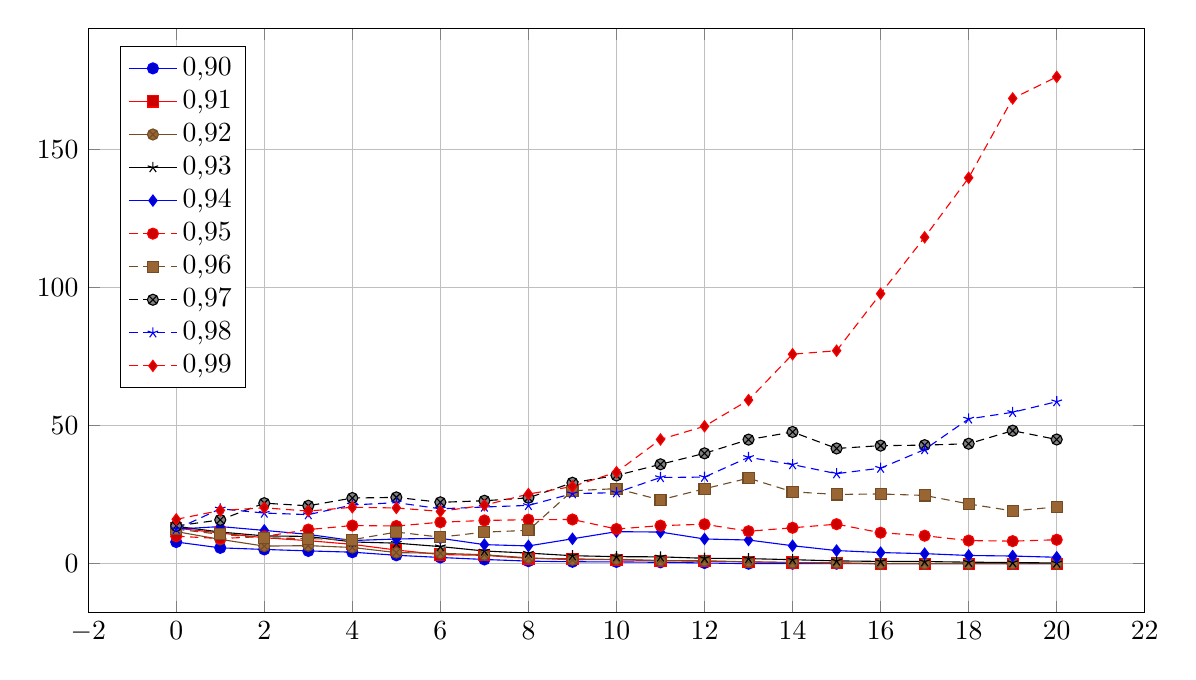
\begin{tikzpicture}
\begin{axis}[
height=9cm,
width=15cm,
grid=major,
legend style = { legend pos = north west }
]
\addplot coordinates {(0, 7.8372054) (1, 5.726038) (2, 5.154667) (3, 4.621181) (4, 4.1600547) (5, 3.0396576) (6, 2.239414) (7, 1.5242789) (8, 0.92045516) (9, 0.6885652) (10, 0.65223116) (11, 0.48610428) (12, 0.2598384) (13, 0.0) (14, 0.0) (15, 0.0) (16, 0.0) (17, 0.0) (18, 0.0) (19, 0.0) (20, 0.0) };
\addlegendentry{0,90}
\addplot coordinates {(0, 12.871898) (1, 11.081771) (2, 9.383892) (3, 8.331373) (4, 6.9849744) (5, 4.9359865) (6, 3.3015344) (7, 3.012378) (8, 1.8939176) (9, 1.7871089) (10, 1.3716524) (11, 1.1143106) (12, 0.8515529) (13, 0.6746103) (14, 0.39734042) (15, 0.20273632) (16, 0.0) (17, 0.0) (18, 0.0) (19, 0.0) (20, 0.0) };
\addlegendentry{0,91}
\addplot coordinates {(0, 11.617334) (1, 8.787009) (2, 6.3560305) (3, 6.531136) (4, 5.861786) (5, 4.0063114) (6, 3.7645807) (7, 3.226793) (8, 2.0987976) (9, 1.3800614) (10, 1.6246796) (11, 1.1037858) (12, 1.059758) (13, 0.6554112) (14, 0.39335263) (15, 0.31620935) (16, 0.0) (17, 0.0) (18, 0.0) (19, 0.0) (20, 0.0) };
\addlegendentry{0,92}
\addplot coordinates {(0, 13.517401) (1, 11.452294) (2, 10.057288) (3, 9.859059) (4, 7.8632793) (5, 7.422488) (6, 6.1805496) (7, 4.5945706) (8, 3.825597) (9, 2.8837724) (10, 2.5438883) (11, 2.4632976) (12, 1.957013) (13, 1.8278275) (14, 1.4445596) (15, 1.0002052) (16, 0.81805015) (17, 0.7711672) (18, 0.5411076) (19, 0.4110637) (20, 0.252428) };
\addlegendentry{0,93}
\addplot coordinates {(0, 12.5) (1, 13.43023) (2, 12.048469) (3, 10.599778) (4, 8.368018) (5, 8.931303) (6, 9.189003) (7, 6.895406) (8, 6.4192615) (9, 9.002274) (10, 11.5897455) (11, 11.443102) (12, 8.935459) (13, 8.56017) (14, 6.4986897) (15, 4.7467318) (16, 4.0223384) (17, 3.6290448) (18, 2.9679754) (19, 2.765107) (20, 2.318351) };
\addlegendentry{0,94}
\addplot coordinates {(0, 9.945217) (1, 9.09356) (2, 9.837457) (3, 12.346309) (4, 13.799155) (5, 13.630574) (6, 14.99853) (7, 15.637733) (8, 15.918938) (9, 15.996337) (10, 12.536006) (11, 13.770408) (12, 14.269985) (13, 11.742347) (14, 12.98971) (15, 14.293675) (16, 11.207167) (17, 10.119975) (18, 8.35863) (19, 8.154236) (20, 8.6633835) };
\addlegendentry{0,95}
\addplot coordinates {(0, 12.5) (1, 10.616831) (2, 9.379364) (3, 9.0645) (4, 8.673918) (5, 11.4384165) (6, 9.595471) (7, 11.418807) (8, 12.055469) (9, 26.387554) (10, 27.160097) (11, 23.074898) (12, 27.107899) (13, 30.953737) (14, 26.003126) (15, 25.055992) (16, 25.225168) (17, 24.703861) (18, 21.618656) (19, 19.09106) (20, 20.514286) };
\addlegendentry{0,96}
\addplot coordinates {(0, 13.680727) (1, 15.846518) (2, 21.887976) (3, 20.95167) (4, 23.759962) (5, 23.993092) (6, 22.206078) (7, 22.775206) (8, 23.825249) (9, 29.290152) (10, 31.927158) (11, 35.96635) (12, 39.931347) (13, 44.896645) (14, 47.657745) (15, 41.694195) (16, 42.71819) (17, 42.896385) (18, 43.41286) (19, 48.133793) (20, 44.937626) };
\addlegendentry{0,97}
\addplot coordinates {(0, 12.5) (1, 19.857609) (2, 18.324724) (3, 17.74957) (4, 21.24073) (5, 22.094864) (6, 19.864298) (7, 20.512543) (8, 21.093626) (9, 25.34785) (10, 25.709059) (11, 31.19894) (12, 31.330263) (13, 38.49805) (14, 35.860638) (15, 32.578533) (16, 34.57723) (17, 41.310635) (18, 52.382793) (19, 54.786243) (20, 58.630527) };
\addlegendentry{0,98}
\addplot coordinates {(0, 16.047285) (1, 19.260551) (2, 20.213194) (3, 19.034306) (4, 20.410967) (5, 20.158894) (6, 18.924496) (7, 21.155848) (8, 25.198473) (9, 27.927269) (10, 33.119106) (11, 44.98241) (12, 49.725594) (13, 59.206253) (14, 75.80497) (15, 77.06952) (16, 97.705864) (17, 118.11795) (18, 139.648) (19, 168.3767) (20, 176.16727) };
\addlegendentry{0,99}
\end{axis}
\end{tikzpicture}



Jak widać w doświadczeniu nie osiągnięto spodziewanych rezultatów. Dla
sprężystości o wartości 1 energia kinetyczna powinna być stała, natomiast tutaj
gwałtownie wzrasta. Wydaje się, że dla utrzymania stałej energii kinetycznej
konieczne jest użycie niższej wartości. Dla polepszenia widoczności poniższy
wykres zawiera wartości energii kinetycznej dla wartości sprężystości od 0,94 do
0,97.

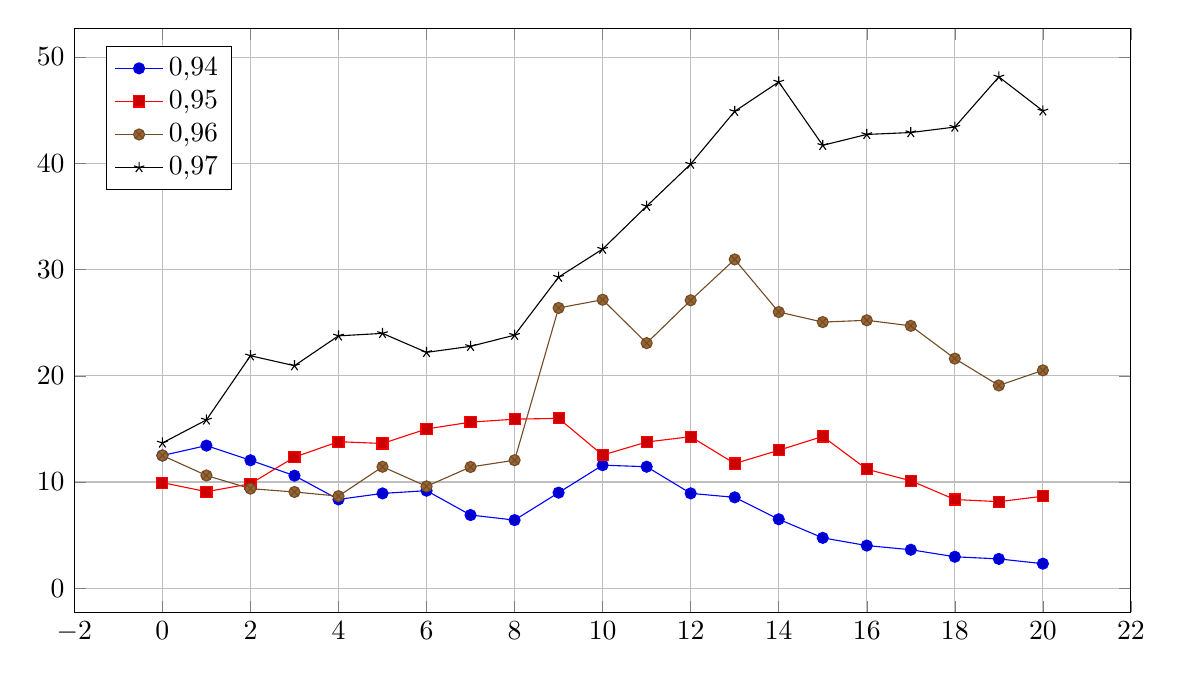
\begin{tikzpicture}
\begin{axis}[
height=9cm,
width=15cm,
grid=major,
legend style = { legend pos = north west }
]
\addplot coordinates {(0, 12.5) (1, 13.43023) (2, 12.048469) (3, 10.599778) (4,8.368018) (5, 8.931303) (6, 9.189003) (7, 6.895406) (8, 6.4192615) (9, 9.002274) (10, 11.5897455) (11, 11.443102) (12, 8.935459) (13, 8.56017) (14, 6.4986897) (15, 4.7467318) (16, 4.0223384) (17, 3.6290448) (18, 2.9679754) (19, 2.765107) (20, 2.318351) };
\addlegendentry{0,94}
\addplot coordinates {(0, 9.945217) (1, 9.09356) (2, 9.837457) (3, 12.346309) (4, 13.799155) (5, 13.630574) (6, 14.99853) (7, 15.637733) (8, 15.918938) (9, 15.996337) (10, 12.536006) (11, 13.770408) (12, 14.269985) (13, 11.742347) (14, 12.98971) (15, 14.293675) (16, 11.207167) (17, 10.119975) (18, 8.35863) (19, 8.154236) (20, 8.6633835) };
\addlegendentry{0,95}
\addplot coordinates {(0, 12.5) (1, 10.616831) (2, 9.379364) (3, 9.0645) (4, 8.673918) (5, 11.4384165) (6, 9.595471) (7, 11.418807) (8, 12.055469) (9, 26.387554) (10, 27.160097) (11, 23.074898) (12, 27.107899) (13, 30.953737) (14, 26.003126) (15, 25.055992) (16, 25.225168) (17, 24.703861) (18, 21.618656) (19, 19.09106) (20, 20.514286) };
\addlegendentry{0,96}
\addplot coordinates {(0, 13.680727) (1, 15.846518) (2, 21.887976) (3, 20.95167) (4, 23.759962) (5, 23.993092) (6, 22.206078) (7, 22.775206) (8, 23.825249) (9, 29.290152) (10, 31.927158) (11, 35.96635) (12, 39.931347) (13, 44.896645) (14, 47.657745) (15, 41.694195) (16, 42.71819) (17, 42.896385) (18, 43.41286) (19, 48.133793) (20, 44.937626) };
\addlegendentry{0,97}
\end{axis}
\end{tikzpicture}



Przy początkowej prędkości 5 m/s i masie 1 kg (linting
\ref{lis:SimpleSnookerScene} ln. 72, 59) energia kinetyczna kulki powinna mieć
stałą wartość energii kinetycznej 12,5.
TODO równanie obliczenia EK.
Z prezentowanego wykresu wynika, że najodpowiedniejsza wartość współczynnika
sprężystości kulki i ścianek mieści się między 0,945 a 0,955.\\
Dla ustalenia bardziej szczegółowej wartości test został powtórzony dla
następujących parametrów z listingu \ref{lis:SimpleSnookerScene}:

\lstinputlisting[language=Java,
  label=lis:SimpleSnookerScene_additional]{./listings/SimpleSnookerScene_additional.java}
  
Ilość odbić została zwiększona dwukrotnie, dzięki czemu możliwe jest sprawdzenie
czy wyrównany poziom energii będzie się utrzymywać.
  
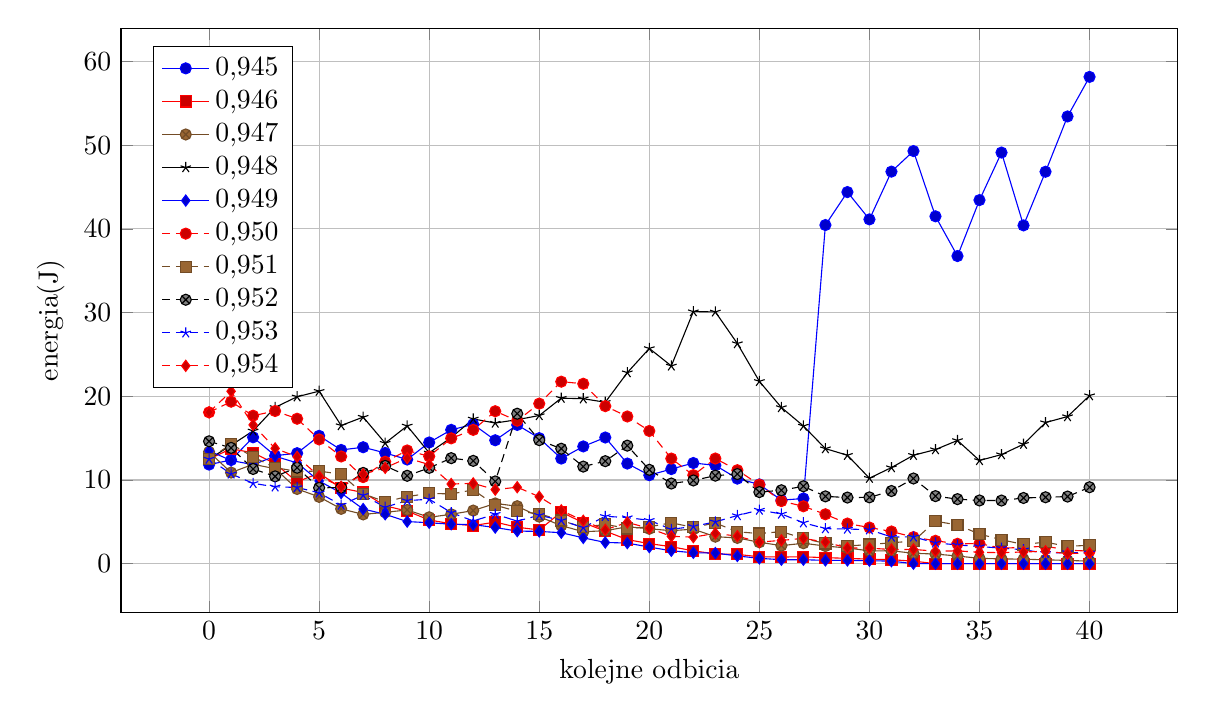
\begin{tikzpicture}
\begin{axis}[
height=9cm,
width=15cm,
grid=major,
xlabel=kolejne odbicia,
ylabel=energia(J),
legend style = { legend pos = north west }
]
\addplot coordinates {(0, 11.83472) (1, 12.379627) (2, 15.0980625) (3, 12.897377) (4, 13.197653) (5, 15.268386) (6, 13.5835) (7, 13.907026) (8, 13.226399) (9, 12.440128) (10, 14.477035) (11, 15.9842) (12, 16.644344) (13, 14.740385) (14, 16.573435) (15, 14.992984) (16, 12.555236) (17, 14.004993) (18, 15.072159) (19, 11.958659) (20, 10.568625) (21, 11.297269) (22, 12.023627) (23, 11.743839) (24, 10.15784) (25, 9.469015) (26, 7.5816555) (27, 7.7853804) (28, 40.450466) (29, 44.389053) (30, 41.125744) (31, 46.831127) (32, 49.287273) (33, 41.49332) (34, 36.746765) (35, 43.43231) (36, 49.10869) (37, 40.409218) (38, 46.817432) (39, 53.422592) (40, 58.14726) };
\addlegendentry{0,945}
\addplot coordinates {(0, 12.5) (1, 13.725066) (2, 13.244118) (3, 11.953949) (4, 9.769774) (5, 10.814914) (6, 9.028812) (7, 8.502626) (8, 6.9107122) (9, 6.27938) (10, 5.2203937) (11, 4.7625675) (12, 4.5451007) (13, 4.9654703) (14, 4.347088) (15, 4.030155) (16, 6.161413) (17, 4.8873606) (18, 3.8916974) (19, 2.8733) (20, 2.3946586) (21, 2.0231962) (22, 1.533896) (23, 1.1654351) (24, 1.111763) (25, 0.82033926) (26, 0.7949642) (27, 0.81605846) (28, 0.7132569) (29, 0.63949037) (30, 0.5374603) (31, 0.4743589) (32, 0.297938) (33, 0.0) (34, 0.0) (35, 0.0) (36, 0.0) (37, 0.0) (38, 0.0) (39, 0.0) (40, 0.0) };
\addlegendentry{0,946}
\addplot coordinates {(0, 13.343076) (1, 10.882678) (2, 11.869106) (3, 11.345713) (4, 8.922309) (5, 7.9773874) (6, 6.547513) (7, 5.882253) (8, 6.130847) (9, 6.4155216) (10, 5.5394745) (11, 5.896995) (12, 6.3431163) (13, 7.1916647) (14, 6.862142) (15, 5.6141715) (16, 4.546112) (17, 3.814531) (18, 3.9349108) (19, 4.4040594) (20, 4.1672707) (21, 3.9381962) (22, 4.1216965) (23, 3.2221136) (24, 3.074441) (25, 2.554985) (26, 2.152308) (27, 2.4376867) (28, 2.1064556) (29, 1.8707508) (30, 1.5296999) (31, 1.5388436) (32, 1.2382075) (33, 1.149339) (34, 0.91256565) (35, 0.63522154) (36, 0.56922203) (37, 0.5338146) (38, 0.45862925) (39, 0.38885325) (40, 0.2969072) };
\addlegendentry{0,947}
\addplot coordinates {(0, 12.5) (1, 14.13552) (2, 15.8612585) (3, 18.670893) (4, 19.937475) (5, 20.604156) (6, 16.50161) (7, 17.508545) (8, 14.396487) (9, 16.455772) (10, 13.244559) (11, 15.055199) (12, 17.29025) (13, 16.797775) (14, 17.200518) (15, 17.697063) (16, 19.771584) (17, 19.701103) (18, 19.285048) (19, 22.817455) (20, 25.708588) (21, 23.621098) (22, 30.10682) (23, 30.076248) (24, 26.296255) (25, 21.77965) (26, 18.656929) (27, 16.446127) (28, 13.739975) (29, 12.953177) (30, 10.209646) (31, 11.477742) (32, 12.947726) (33, 13.629319) (34, 14.718304) (35, 12.328139) (36, 13.029368) (37, 14.271083) (38, 16.854652) (39, 17.572474) (40, 20.073355) };
\addlegendentry{0,948}
\addplot coordinates {(0, 13.470681) (1, 12.325375) (2, 11.826186) (3, 12.835963) (4, 12.031693) (5, 9.875669) (6, 8.433987) (7, 6.5284123) (8, 5.901152) (9, 5.0297904) (10, 4.8878074) (11, 4.7115064) (12, 4.658539) (13, 4.315971) (14, 3.8937955) (15, 3.852501) (16, 3.6964788) (17, 3.084705) (18, 2.5341594) (19, 2.460717) (20, 1.9807745) (21, 1.5402061) (22, 1.3024533) (23, 1.2666614) (24, 0.92073756) (25, 0.6371743) (26, 0.47197518) (27, 0.4704443) (28, 0.39559248) (29, 0.38954863) (30, 0.35554305) (31, 0.29937363) (32, 0.0) (33, 0.0) (34, 0.0) (35, 0.0) (36, 0.0) (37, 0.0) (38, 0.0) (39, 0.0) (40, 0.0) };
\addlegendentry{0,949}
\addplot coordinates {(0, 18.075089) (1, 19.348585) (2, 17.674715) (3, 18.23503) (4, 17.312439) (5, 14.840965) (6, 12.803486) (7, 10.340366) (8, 12.173147) (9, 13.52262) (10, 12.823664) (11, 14.969939) (12, 15.979581) (13, 18.209831) (14, 17.077518) (15, 19.11712) (16, 21.73974) (17, 21.490181) (18, 18.81594) (19, 17.580912) (20, 15.849103) (21, 12.554693) (22, 10.572047) (23, 12.559721) (24, 11.165561) (25, 9.431433) (26, 7.4705954) (27, 6.854054) (28, 5.899695) (29, 4.790389) (30, 4.3167667) (31, 3.8425434) (32, 3.17302) (33, 2.7332091) (34, 2.3748143) (35, 2.3970597) (36, 1.84973) (37, 1.9432095) (38, 2.087145) (39, 1.6142488) (40, 1.4980283) };
\addlegendentry{0,950}
\addplot coordinates {(0, 12.5) (1, 14.287379) (2, 12.751261) (3, 11.474439) (4, 11.014549) (5, 11.059993) (6, 10.678994) (7, 8.348292) (8, 7.3942523) (9, 8.00856) (10, 8.404354) (11, 8.3236065) (12, 8.814266) (13, 6.9876337) (14, 6.250312) (15, 5.9692373) (16, 5.1552496) (17, 4.34337) (18, 4.697723) (19, 4.2021036) (20, 4.4029956) (21, 4.88272) (22, 4.3309884) (23, 4.8590584) (24, 3.806094) (25, 3.5954096) (26, 3.8256135) (27, 3.019442) (28, 2.412923) (29, 2.1122441) (30, 2.2830546) (31, 2.4955637) (32, 2.6976843) (33, 5.0676746) (34, 4.630739) (35, 3.531819) (36, 2.855678) (37, 2.2971077) (38, 2.5723886) (39, 2.0594285) (40, 2.205233) };
\addlegendentry{0,951}
\addplot coordinates {(0, 14.615244) (1, 13.829683) (2, 11.311698) (3, 10.427009) (4, 11.460272) (5, 9.057038) (6, 9.099048) (7, 10.840954) (8, 11.678121) (9, 10.499791) (10, 11.441355) (11, 12.603779) (12, 12.279609) (13, 9.823079) (14, 17.913473) (15, 14.754623) (16, 13.729808) (17, 11.595872) (18, 12.243206) (19, 14.099075) (20, 11.214356) (21, 9.572169) (22, 9.937819) (23, 10.514322) (24, 10.702424) (25, 8.548818) (26, 8.768956) (27, 9.24096) (28, 8.037726) (29, 7.8958397) (30, 7.919593) (31, 8.676345) (32, 10.173832) (33, 8.067685) (34, 7.7079425) (35, 7.548844) (36, 7.5379424) (37, 7.846434) (38, 7.9307866) (39, 8.014059) (40, 9.130319) };
\addlegendentry{0,952}
\addplot coordinates {(0, 12.5) (1, 10.7275) (2, 9.595271) (3, 9.179574) (4, 9.106409) (5, 8.454757) (6, 7.0024796) (7, 8.17677) (8, 6.750139) (9, 7.5269756) (10, 7.698658) (11, 6.103392) (12, 5.0972943) (13, 5.914313) (14, 5.076894) (15, 5.787914) (16, 5.162111) (17, 4.3161173) (18, 5.6562753) (19, 5.5016747) (20, 5.1850286) (21, 4.1028576) (22, 4.4445443) (23, 4.9968286) (24, 5.750374) (25, 6.4052725) (26, 5.936255) (27, 4.8863425) (28, 4.1847186) (29, 4.1409235) (30, 4.0526757) (31, 3.1830995) (32, 3.1974099) (33, 2.4858365) (34, 2.2343047) (35, 2.0511215) (36, 1.8490995) (37, 1.6669159) (38, 1.2392174) (39, 1.3421869) (40, 1.2746574) };
\addlegendentry{0,953}
\addplot coordinates {(0, 18.07279) (1, 20.592321) (2, 16.581625) (3, 13.767898) (4, 12.763923) (5, 10.439662) (6, 9.18948) (7, 10.687139) (8, 11.447489) (9, 12.615019) (10, 11.8371315) (11, 9.515284) (12, 9.591186) (13, 8.840663) (14, 9.133119) (15, 7.9945536) (16, 6.3630214) (17, 5.123591) (18, 4.040571) (19, 4.926172) (20, 4.223811) (21, 3.267189) (22, 3.1675262) (23, 3.6172326) (24, 3.2864053) (25, 2.576568) (26, 2.7800326) (27, 3.020876) (28, 2.5800412) (29, 1.8733292) (30, 1.85761) (31, 1.6878184) (32, 1.7023418) (33, 1.4894247) (34, 1.5277467) (35, 1.3547096) (36, 1.3137895) (37, 1.3966576) (38, 1.4822598) (39, 1.2024833) (40, 1.2677329) };
\addlegendentry{0,954}
\end{axis}
\end{tikzpicture}

Jak widać poziom energii nie utrzymuje się dla zwiększonej ilości odbić. W
dodatku w losowych momentach (na prezentowanym wykresie dla wartości
współczynnika sprężystości 0,945 dla 27. odbicia) można zaobserwować jego
gwałtowne wzrosty. Dla złagodzenia efektów tych wzrostów na poniższym wykresie
przedstawiono uśredniony wynik dziesięciu testów.

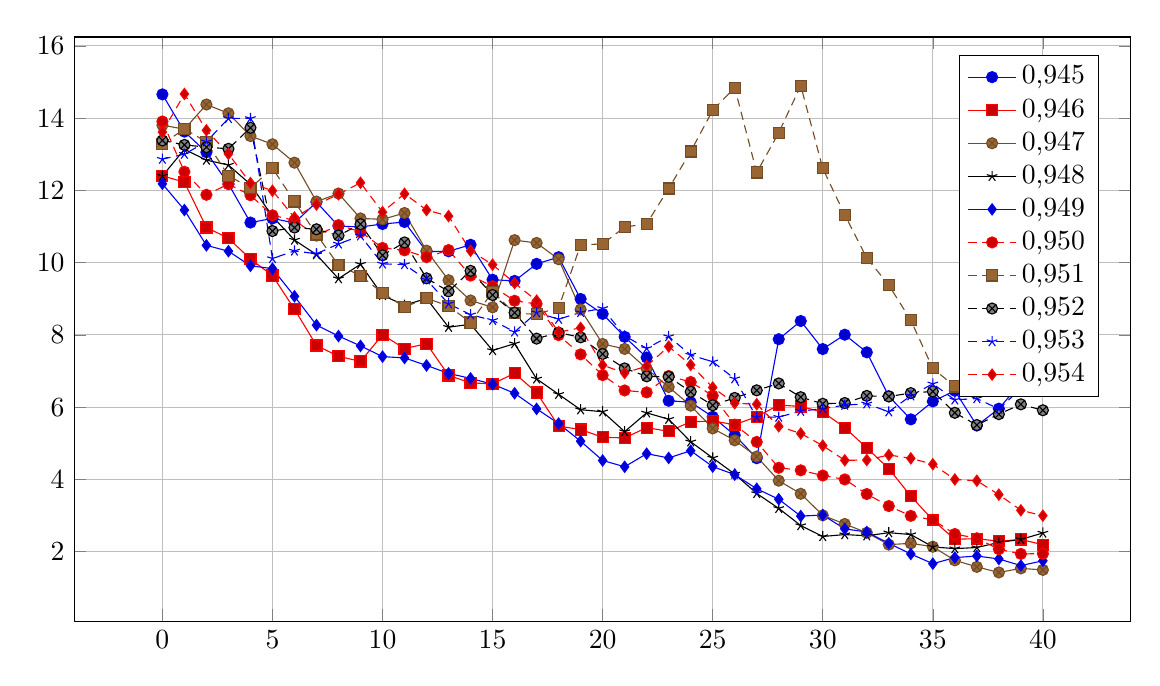
\begin{tikzpicture}
\begin{axis}[
height=9cm,
width=15cm,
grid=major,
legend style = { legend pos = north east }
]
\addplot coordinates {(0, 14.6562260627747) (1, 13.6256645202637) (2, 13.054486989975) (3, 12.1763894557953) (4, 11.108833360672) (5, 11.2233946323395) (6, 11.0991048336029) (7, 11.6744068145752) (8, 11.0118092298508) (9, 10.9873273611069) (10, 11.0685114145279) (11, 11.1239978551865) (12, 10.3053623557091) (13, 10.3141089200974) (14, 10.4938254594803) (15, 9.52750028371811) (16, 9.49386215209961) (17, 9.96602758169174) (18, 10.1507727026939) (19, 8.99497901201248) (20, 8.58136545419693) (21, 7.94662589430809) (22, 7.37444679141045) (23, 6.17753539681435) (24, 6.13745829164982) (25, 5.73345747590065) (26, 5.22426048517227) (27, 4.58836826682091) (28, 7.8813433110714) (29, 8.38399687707424) (30, 7.6084086805582) (31, 8.00572631806135) (32, 7.51851252317429) (33, 6.30226357579231) (34, 5.66303240656853) (35, 6.16019782423973) (36, 6.45491213798523) (37, 5.49251633584499) (38, 5.9576107352972) (39, 6.67393660545349) (40, 6.9803785264492) };
\addlegendentry{0,945}
\addplot coordinates {(0, 12.4022218704224) (1, 12.2259508132935) (2, 10.9725129127502) (3, 10.6760525226593) (4, 10.0991243362427) (5, 9.64306182861328) (6, 8.71197805404663) (7, 7.70718474388123) (8, 7.40868282318115) (9, 7.26591448783874) (10, 8.00451288223267) (11, 7.62072007656097) (12, 7.75652910470963) (13, 6.87890261411667) (14, 6.672678399086) (15, 6.64590454101563) (16, 6.93818979263306) (17, 6.40504869222641) (18, 5.47706761956215) (19, 5.38112026453018) (20, 5.16761724352837) (21, 5.14959081411362) (22, 5.43434517979622) (23, 5.33113816380501) (24, 5.59545066356659) (25, 5.61735334992409) (26, 5.51616925597191) (27, 5.73644617795944) (28, 6.06001359522343) (29, 6.01864603757858) (30, 5.86524453163147) (31, 5.43487996459007) (32, 4.8719010040164) (33, 4.30030767023563) (34, 3.53826675415039) (35, 2.87623463273048) (36, 2.34437598586082) (37, 2.36291944980621) (38, 2.29072198867798) (39, 2.33935695886612) (40, 2.19480673074722) };
\addlegendentry{0,946}
\addplot coordinates {(0, 13.8043006896973) (1, 13.6925736427307) (2, 14.3758071422577) (3, 14.1325853347778) (4, 13.5025720119476) (5, 13.2755349636078) (6, 12.7663237094879) (7, 11.6888662338257) (8, 11.9123019456863) (9, 11.2239685535431) (10, 11.1973436832428) (11, 11.3732707977295) (12, 10.3317072629929) (13, 9.51320831775665) (14, 8.95262567996979) (15, 8.76283481121063) (16, 10.6224771022797) (17, 10.5448018312454) (18, 10.0935352087021) (19, 8.7033514380455) (20, 7.7492377281189) (21, 7.61283913850784) (22, 7.06518988609314) (23, 6.559628033638) (24, 6.04167060852051) (25, 5.41185646653175) (26, 5.08241978287697) (27, 4.63394111096859) (28, 3.96660267710686) (29, 3.60402843356133) (30, 3.00693404078484) (31, 2.76765021979809) (32, 2.52679316997528) (33, 2.19694601595402) (34, 2.23208404928446) (35, 2.13959696292877) (36, 1.76221565306187) (37, 1.58085741400719) (38, 1.42672650814056) (39, 1.53932392001152) (40, 1.49729729890823) };
\addlegendentry{0,947}
\addplot coordinates {(0, 12.3982768058777) (1, 13.1348707199097) (2, 12.8372737884521) (3, 12.7001321792603) (4, 12.1672739028931) (5, 11.2750558376312) (6, 10.6261374473572) (7, 10.221337556839) (8, 9.55598180294037) (9, 9.95648241043091) (10, 9.09451639652252) (11, 8.82288656234741) (12, 9.00808305740356) (13, 8.21335928440094) (14, 8.29480786323547) (15, 7.57112445831299) (16, 7.75750745534897) (17, 6.78246188163757) (18, 6.35715628862381) (19, 5.93029171228409) (20, 5.87394794225693) (21, 5.32377170324326) (22, 5.8426962852478) (23, 5.66730691492558) (24, 5.04262288212776) (25, 4.59558297395706) (26, 4.14988817870617) (27, 3.61246277689934) (28, 3.19977921843529) (29, 2.72453445792198) (30, 2.42193761765957) (31, 2.47530001997948) (32, 2.44172253012657) (33, 2.52722045183182) (34, 2.47533693313599) (35, 2.13422930836678) (36, 2.08558965623379) (37, 2.11694244146347) (38, 2.25741191506386) (39, 2.34004321694374) (40, 2.51835238933563) };
\addlegendentry{0,948}
\addplot coordinates {(0, 12.1814444541931) (1, 11.4556957244873) (2, 10.4778209686279) (3, 10.3164783477783) (4, 9.91166429519653) (5, 9.83501195907593) (6, 9.06741237640381) (7, 8.27128520011902) (8, 7.96847171783447) (9, 7.6957754611969) (10, 7.39932823181152) (11, 7.36326403617859) (12, 7.15495343208313) (13, 6.93551654815674) (14, 6.79657573699951) (15, 6.63643126487732) (16, 6.38545722961426) (17, 5.95384972095489) (18, 5.54752365350723) (19, 5.0591068983078) (20, 4.52486710548401) (21, 4.35102623701096) (22, 4.71317600607872) (23, 4.59588846564293) (24, 4.79488226175308) (25, 4.35584520101547) (26, 4.1336768835783) (27, 3.74193927943706) (28, 3.45298179388046) (29, 2.98590224385262) (30, 3.01562243700027) (31, 2.63291162550449) (32, 2.54467267990112) (33, 2.23404234349728) (34, 1.9367674946785) (35, 1.66969993859529) (36, 1.83733677864075) (37, 1.88249142169952) (38, 1.79945760965347) (39, 1.61711151599884) (40, 1.74928727149963) };
\addlegendentry{0,949}
\addplot coordinates {(0, 13.9059829711914) (1, 12.5137694358826) (2, 11.8774974822998) (3, 12.1741494178772) (4, 11.8651987075806) (5, 11.310263633728) (6, 11.1685515403748) (7, 10.7494470119476) (8, 11.0378528118134) (9, 10.8539872646332) (10, 10.4069371700287) (11, 10.339888048172) (12, 10.1519442081451) (13, 10.3484754562378) (14, 9.64128794670105) (15, 9.3442617893219) (16, 8.94458522796631) (17, 8.85833351612091) (18, 7.99419071674347) (19, 7.46127936840057) (20, 6.88672922849655) (21, 6.46321547031403) (22, 6.40967074632645) (23, 6.86291975975037) (24, 6.69745423793793) (25, 6.31787598729134) (26, 5.51692352890968) (27, 5.03974458575249) (28, 4.32343353331089) (29, 4.25268172323704) (30, 4.10942476689816) (31, 4.00075962543488) (32, 3.59627936184406) (33, 3.26424064040184) (34, 2.99327031373978) (35, 2.88445642590523) (36, 2.49013569056988) (37, 2.37197640538216) (38, 2.06999402344227) (39, 1.94008515179157) (40, 1.94661874473095) };
\addlegendentry{0,950}
\addplot coordinates {(0, 13.2781973838806) (1, 13.7021299362183) (2, 13.3391201972961) (3, 12.4054169178009) (4, 12.0662398815155) (5, 12.6113337993622) (6, 11.6933528900146) (7, 10.780289888382) (8, 9.93317956924438) (9, 9.63696854114533) (10, 9.15944323539734) (11, 8.77189693450928) (12, 9.0159517288208) (13, 8.79784791469574) (14, 8.34251778125763) (15, 9.19578952789307) (16, 8.59856331348419) (17, 8.57238194942474) (18, 8.753364610672) (19, 10.4900251150131) (20, 10.5187027931213) (21, 10.9836204528809) (22, 11.075525021553) (23, 12.0515645503998) (24, 13.0754309654236) (25, 14.2149050116539) (26, 14.8429864764214) (27, 12.4947864532471) (28, 13.5947657942772) (29, 14.8968303561211) (30, 12.6081966876984) (31, 11.3213147640228) (32, 10.1299663484097) (33, 9.37871618270874) (34, 8.40511998534203) (35, 7.07489039599895) (36, 6.57302742898464) (37, 6.92401961386204) (38, 7.54064406454563) (39, 6.66278366148472) (40, 8.08269311785698) };
\addlegendentry{0,951}
\addplot coordinates {(0, 13.3815976142883) (1, 13.2575705528259) (2,13.1966584205627) (3, 13.1495709896088) (4, 13.7313847064972) (5, 10.8742453098297) (6, 10.9705602645874) (7, 10.9229876279831) (8, 10.7496512889862) (9, 11.0642107725143) (10, 10.2030373573303) (11, 10.5597208023071) (12, 9.56631820201874) (13, 9.204722905159) (14, 9.77342791557312) (15, 9.10343494415283) (16, 8.61196794509888) (17, 7.89711513519287) (18, 8.06343204975128) (19, 7.93230175971985) (20, 7.47169940471649) (21, 7.07361674308777) (22, 6.85348105430603) (23, 6.83944536447525) (24, 6.42703374624252) (25, 6.05213391780853) (26, 6.25701947212219) (27, 6.46634848117828) (28, 6.65723429918289) (29, 6.27693936228752) (30, 6.09445922374725) (31, 6.11582781076431) (32, 6.31241797208786) (33, 6.2971722304821) (34, 6.38925131559372) (35, 6.43648965060711) (36, 5.84381370544434) (37, 5.5056351006031) (38, 5.80657843947411) (39, 6.07883229255676) (40, 5.91480894088745) };
\addlegendentry{0,952}
\addplot coordinates {(0, 12.8636241912842) (1, 13.0021504402161) (2,
13.3448638916016) (3, 13.9903785705566) (4, 13.9917116641998) (5,
10.1146651744843) (6, 10.3231254577637) (7, 10.2456952095032) (8, 10.5174011230469) (9, 10.7428637504578) (10, 9.96562452316284) (11, 9.94694910049438) (12, 9.52446849346161) (13, 8.86221284866333) (14, 8.55821604728699) (15, 8.40437412261963) (16, 8.08280463218689) (17, 8.61760497093201) (18, 8.43606390953064) (19, 8.62183849811554) (20, 8.73446414470673) (21, 7.97404136657715) (22, 7.62777805328369) (23, 7.95511655807495) (24, 7.44362692832947) (25, 7.25623573064804) (26, 6.7876464009285) (27, 5.71654962301254) (28, 5.7262363910675) (29, 5.88920958042145) (30, 5.95987671017647) (31, 6.05756386518478) (32, 6.09318507313728) (33, 5.87254739105701) (34, 6.31689597964287) (35, 6.6472687035799) (36, 6.20203223526478) (37, 6.23965192735195) (38, 5.95067174732685) (39, 6.51158805936575) (40, 7.11151877641678) };
\addlegendentry{0,953}
\addplot coordinates {(0, 13.6133923530579) (1, 14.6667778968811) (2, 13.6618516921997) (3, 13.0073251724243) (4, 12.2023746013641) (5, 11.9906059265137) (6, 11.2490232944489) (7, 11.6071300029755) (8, 11.8916132926941) (9, 12.2103487968445) (10, 11.3969748973846) (11, 11.9060091018677) (12, 11.4559844017029) (13, 11.2876661777496) (14, 10.3291625261307) (15, 9.94409117698669) (16, 9.43445086479187) (17, 8.94726392030716) (18, 8.0772367477417) (19, 8.19570999145508) (20, 7.16313669681549) (21, 6.94529861211777) (22, 7.13770437240601) (23, 7.67992736101151) (24, 7.16948624849319) (25, 6.5456313252449) (26, 6.10883691906929) (27, 6.082444190979) (28, 5.47121298313141) (29, 5.27222081124783) (30, 4.93714967370033) (31, 4.5299041301012) (32, 4.53709046840668) (33, 4.67730629444122) (34, 4.58505046367645) (35, 4.42233805656433) (36, 4.00028142035007) (37, 3.96476039290428) (38, 3.58045221269131) (39, 3.14697138667107) (40, 2.99718299508095) };
\addlegendentry{0,954}
\end{axis}
\end{tikzpicture}


Spadki wartości energii kinetycznych sugerują, że nawet przy początkowo dobrze
dobranych współczynnikach sprężystości, przy większej ilości odbić energia nie
utrzymuje stałej wartości. Przy wartości współczynnika równej jedności energia
nie utrzymuje stałej wartości, a wzrasta. Co jest tego przyczyną? \\
W poszukiwaniu odpowiedzi na to pytanie można spojrzeć na wyniki poprzednich
testów rozpatrując osobno zapisy energii kinetycznej liniowej i obrotowej.
Poniżej przedstawiono fragment zapisu dla testu przy watrości współczynnika
sprężystości 0,98:

\lstinputlisting[language=xml, caption=wartości energii kinetycznej,
  label=lis:manifest,linerange={6-12}]{./listings/0,98.txt}
  
Można zaobserwować gwałtowne zmiany obu energii, jednak wzrost energii
kinetycznej liniowej jest zawsze poprzedzony wzrostem energii kinetycznej
obrotowej. Liniowa energia kinetyczna sama w sobie nie ulega gwałtownym
wzrostom. Przyczyną tego jest wzrost energii całkowitej.\\
Podczas analitycznego rozważania odbicia ciała możliwe jest dokładne ustalenie
czasu i miejsca zderzenia poprzez rozwiązanie odpowiedniego równania ruchu. W
przypadku symulacji zderzenia ciał przez silnik fizyczny, symulacja ta jest
dzielona na kroki. Każdy krok odpowiada minięciu kwantu czasu o z góry ustalonej
wartości i wszystkie ciała uczestniczące w symulacji poruszają się adekwatnie do
swojej prędkości. Prawie niemożliwe jest więc uzyskanie sytuacji w której
zderzenie powierzchni sferycznej z płaską będzie tylko jednym punktem.

\begin{center}
\includegraphics{./img/zderzenie1.png}
\end{center}

W przypadku zderzenia w symulacji zderzenie nie jest punktem a powierzchnią.
Silnik bullet do obliczenia parametrów reakcji na zderzenie potrzebuje
określenia obszaru zderzenia jako punktu (który jest wybrany z powierzchni
obszaru zderzenia oznaczonego na poniższej ilustracji czerwoną linią). Niestety
im większy jest obszar zderzenia tym większe jest prawdopodobieństwo błędu w
wyborze odpowiedniego punktu. Przesunięcie tego punktu względem właściwego
umiejscowienia pozycji zderzenia wynikające z niedokładności obliczeniowej
decyduje o nadmiarze lub niedoborze obrotowej energii kinetycznej.

\begin{center}
\includegraphics{./img/zderzenie2.png}
\end{center}

Aby zminimalizować możliwą wielkość obszaru zderzenia można zmniejszyć kwant
czasu, minimalizując odległości przebywane przez ciała w każdym kroku
symulacji.\\
Aby tego dokonać należy przyjrzeć się prototypowi funkcji \emph{stepSimulation}.

\lstinputlisting[language=c++,
label=lis:stepSimulation]{./listings/stepSimulation.cpp}

Funkcja ta jest wywoływana w celu zaktualizowania symulacji o pewien
czas(wywoływana jest dla każdej renderowanej klatki aplikacji). Według
\emph{Bullet User Manual}(TODO:źródło z bibliografii) jej poszczególne parametry
oznaczają:\\
\\
\textbf{timeStep}: całkowita ilość czasu jaka musi minąć w danym kroku. W
symulacjach jest to najczęściej odstęp czasu pomiędzy wyświetleniem poprzedniej
i następnej klatki.\\
\textbf{fixedTimeStep}: silnik Bullet każdy krok symulacji dzieli na podkroki o
długości okreslanej tym parametrem. To właśnie ten parametr decyduje o
dokładności symulacji. Jeśli \emph{timeStep} jest mniejsze od
\emph{fixedTimeStep} ruch ciał zostaje interpolowany. Domyślna wartość parametru
to $ \frac{1}{60} $ sekundy.\\
\textbf{maxSubSteps}: czasem z powodu spowolnień pracy silnika lub aplikacji
wartość \emph{timeStep} może być bardzo duża. Aby zapobiec zbyt dużym przeskokom
w animacji parametr ten określa maksymalną ilość podkroków jakie mogą być
wykonane w jednym kroku symulacji. Innymi słowy relacja parametrów powinna
wyglądać następująco:\\
$ timeStep < fixedTimeStep * maxSubSteps $

Domyślną wartością \emph{maxSubSteps} jest 1.

Kolejnym testem jest zmodyfikowany test z listingu \ref{lis:SimpleSnookerScene}.
Tym razem nie jest badana zależność energii kinetycznej od współczynnika
sprężystości, a od parametru \emph{fixedTimeStep}. 

\lstinputlisting[language=Java,
  label=lis:SimpleSnookerSceneFts,caption=scena
  testująca zależność energii
  kinetycznej od fixedTimeStep]{./listings/SimpleSnookerSceneFts.java}

Zależność energii kinetycznej od odbicia(poszczególne linie wykresu
reprezentują wartości współczynnika ftsFactor). Dla czytelności wykresu $
fixedTimeStep = \frac{1}{ftsFactor} $. Współczynnik sprężystości został
ustawiony na 1. Prędkość ciała wynosi 5$\frac{m}{s}$.

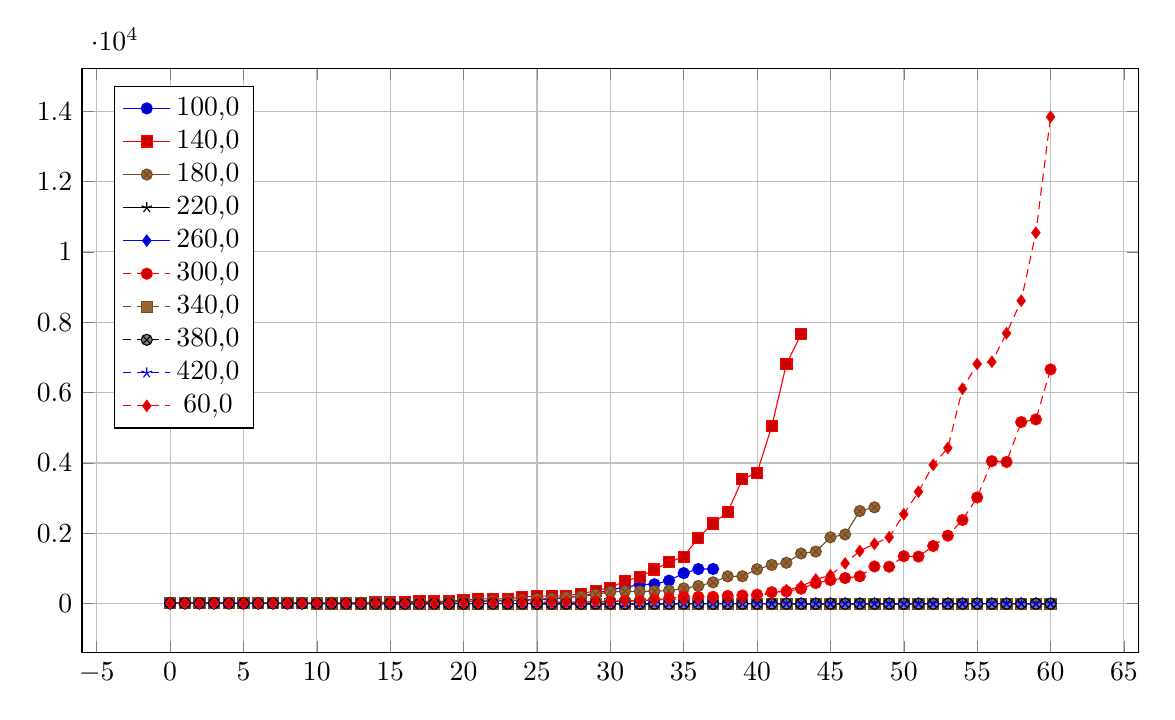
\begin{tikzpicture}
\begin{axis}[
height=9cm,
width=15cm,
grid=major,
legend style = { legend pos = north west }
]
\addplot coordinates {(0, 12.5 ) (1, 12.49999 ) (2, 12.499824 ) (3, 12.498202 ) (4, 12.481768 ) (5, 12.316477 ) (6, 15.795458 ) (7, 15.392218 ) (8, 15.434127 ) (9, 15.410436 ) (10, 15.239715 ) (11, 20.11805 ) (12, 19.633654 ) (13, 20.956968 ) (14, 22.878029 ) (15, 31.070366 ) (16, 38.64726 ) (17, 39.382668 ) (18, 52.701916 ) (19, 52.103355 ) (20, 63.929455 ) (21, 74.69516 ) (22, 79.91147 ) (23, 81.80447 ) (24, 95.30267 ) (25, 116.33796 ) (26, 122.753006 ) (27, 171.626 ) (28, 225.77719 ) (29, 282.66235 ) (30, 402.16544 ) (31, 462.3927 ) (32, 545.8912 ) (33, 554.0528 ) (34, 657.7108 ) (35, 869.9793 ) (36, 985.12476 ) (37, 987.26605 ) };
\addlegendentry{100,0}
\addplot coordinates {(0, 12.5 ) (1, 12.499967 ) (2, 12.499719 ) (3, 12.496181 ) (4, 12.446304 ) (5, 11.755087 ) (6, 11.572497 ) (7, 12.945028 ) (8, 12.642736 ) (9, 15.052362 ) (10, 13.829583 ) (11, 17.761051 ) (12, 22.982285 ) (13, 30.615692 ) (14, 38.457775 ) (15, 47.436565 ) (16, 58.842197 ) (17, 64.2831 ) (18, 62.14132 ) (19, 80.48335 ) (20, 108.55065 ) (21, 133.80923 ) (22, 139.68195 ) (23, 137.094 ) (24, 191.534 ) (25, 219.08894 ) (26, 215.14224 ) (27, 230.26402 ) (28, 281.01144 ) (29, 373.2563 ) (30, 456.31274 ) (31, 643.2415 ) (32, 765.12286 ) (33, 972.59406 ) (34, 1176.4192 ) (35, 1337.1683 ) (36, 1875.6881 ) (37, 2279.3777 ) (38, 2609.1792 ) (39, 3538.376 ) (40, 3725.553 ) (41, 5041.8345 ) (42, 6811.656 ) (43, 7661.2676 ) };
\addlegendentry{140,0}
\addplot coordinates {(0, 12.5 ) (1, 12.500086 ) (2, 12.501545 ) (3, 12.527953 ) (4, 13.00956 ) (5, 16.828875 ) (6, 15.706829 ) (7, 15.004946 ) (8, 14.830004 ) (9, 17.307192 ) (10, 18.304008 ) (11, 22.046404 ) (12, 20.210443 ) (13, 23.944548 ) (14, 29.67809 ) (15, 30.661171 ) (16, 36.484932 ) (17, 35.100254 ) (18, 40.778275 ) (19, 55.056026 ) (20, 64.672775 ) (21, 65.86728 ) (22, 87.03496 ) (23, 95.66851 ) (24, 104.94852 ) (25, 137.02641 ) (26, 147.80406 ) (27, 188.14395 ) (28, 206.13316 ) (29, 259.87714 ) (30, 339.46973 ) (31, 353.81726 ) (32, 351.1574 ) (33, 356.59348 ) (34, 372.64868 ) (35, 435.89276 ) (36, 505.09164 ) (37, 608.1733 ) (38, 777.6239 ) (39, 781.0758 ) (40, 980.99603 ) (41, 1103.1704 ) (42, 1163.442 ) (43, 1428.3059 ) (44, 1482.0144 ) (45, 1887.713 ) (46, 1969.0378 ) (47, 2634.8774 ) (48, 2739.9836 ) };
\addlegendentry{180,0}
\addplot coordinates {(0, 12.5 ) (1, 12.499971 ) (2, 12.498856 ) (3, 12.470235 ) (4, 11.736132 ) (5, 11.689475 ) (6, 9.801909 ) (7, 8.49379 ) (8, 7.395703 ) (9, 8.466985 ) (10, 7.53862 ) (11, 7.24089 ) (12, 8.123841 ) (13, 6.475091 ) (14, 6.414579 ) (15, 5.3106594 ) (16, 5.4164762 ) (17, 4.3162026 ) (18, 3.296064 ) (19, 2.739808 ) (20, 2.5333169 ) (21, 1.987436 ) (22, 1.6969215 ) (23, 1.4240198 ) (24, 1.0527757 ) (25, 0.6289513 ) (26, 0.38676772 ) (27, 0.17112246 ) (28, 0.0 ) (29, 0.0 ) (30, 0.0 ) (31, 0.0 ) (32, 0.0 ) (33, 0.0 ) (34, 0.0 ) (35, 0.0 ) (36, 0.0 ) (37, 0.0 ) (38, 0.0 ) (39, 0.0 ) (40, 0.0 ) (41, 0.0 ) (42, 0.0 ) (43, 0.0 ) (44, 0.0 ) (45, 0.0 ) (46, 0.0 ) (47, 0.0 ) (48, 0.0 ) (49, 0.0 ) (50, 0.0 ) (51, 0.0 ) (52, 0.0 ) (53, 0.0 ) (54, 0.0 ) (55, 0.0 ) (56, 0.0 ) (57, 0.0 ) (58, 0.0 ) (59, 0.0 ) (60, 0.0 ) };
\addlegendentry{220,0}
\addplot coordinates {(0, 12.5 ) (1, 12.5 ) (2, 12.5 ) (3, 12.5 ) (4, 12.5 ) (5, 12.5 ) (6, 12.5 ) (7, 12.5 ) (8, 12.5 ) (9, 12.5 ) (10, 12.5 ) (11, 12.5 ) (12, 12.5 ) (13, 12.5 ) (14, 12.5 ) (15, 12.5 ) (16, 12.5 ) (17, 12.5 ) (18, 12.5 ) (19, 12.5 ) (20, 12.5 ) (21, 12.5 ) (22, 12.5 ) (23, 12.5 ) (24, 12.5 ) (25, 12.5 ) (26, 12.5 ) (27, 12.5 ) (28, 12.5 ) (29, 12.5 ) (30, 12.5 ) (31, 12.5 ) (32, 12.5 ) (33, 12.5 ) (34, 12.5 ) (35, 12.5 ) (36, 12.5 ) (37, 12.5 ) (38, 12.5 ) (39, 12.5 ) (40, 12.5 ) (41, 12.5 ) (42, 12.5 ) (43, 12.5 ) (44, 12.5 ) (45, 12.5 ) (46, 12.5 ) (47, 12.5 ) (48, 12.5 ) (49, 12.5 ) (50, 12.5 ) (51, 12.5 ) (52, 12.5 ) (53, 12.5 ) (54, 12.5 ) (55, 12.5 ) (56, 12.5 ) (57, 12.5 ) (58, 12.5 ) (59, 12.5 ) (60, 12.5 ) };
\addlegendentry{260,0}
\addplot coordinates {(0, 12.499857 ) (1, 12.495675 ) (2, 12.370698 ) (3, 13.60359 ) (4, 13.500814 ) (5, 11.857204 ) (6, 13.439519 ) (7, 13.624933 ) (8, 15.260229 ) (9, 15.055403 ) (10, 17.272354 ) (11, 17.70488 ) (12, 17.010616 ) (13, 20.71158 ) (14, 20.718487 ) (15, 24.961153 ) (16, 29.187761 ) (17, 34.821487 ) (18, 30.847595 ) (19, 28.75227 ) (20, 32.012222 ) (21, 32.095547 ) (22, 37.203342 ) (23, 48.29855 ) (24, 49.83079 ) (25, 45.833984 ) (26, 43.64385 ) (27, 41.03238 ) (28, 47.254562 ) (29, 57.411808 ) (30, 70.60043 ) (31, 82.11667 ) (32, 85.857285 ) (33, 109.84031 ) (34, 148.7622 ) (35, 201.23523 ) (36, 194.39172 ) (37, 198.31165 ) (38, 222.07056 ) (39, 234.42426 ) (40, 256.3978 ) (41, 328.6761 ) (42, 350.54938 ) (43, 426.6949 ) (44, 585.76324 ) (45, 671.96454 ) (46, 729.54614 ) (47, 778.2264 ) (48, 1058.2607 ) (49, 1052.0831 ) (50, 1350.322 ) (51, 1340.2926 ) (52, 1641.1189 ) (53, 1933.7147 ) (54, 2379.2126 ) (55, 3022.0554 ) (56, 4051.6084 ) (57, 4029.8694 ) (58, 5162.7783 ) (59, 5238.7476 ) (60, 6661.5063 ) };
\addlegendentry{300,0}
\addplot coordinates {(0, 12.5 ) (1, 12.500324 ) (2, 12.510459 ) (3, 12.8578205 ) (4, 14.523903 ) (5, 14.485657 ) (6, 14.996248 ) (7, 13.288555 ) (8, 10.443586 ) (9, 9.050881 ) (10, 7.6211677 ) (11, 6.8238263 ) (12, 7.3748183 ) (13, 5.9362407 ) (14, 5.6662164 ) (15, 4.837941 ) (16, 3.3367136 ) (17, 2.1178775 ) (18, 1.5461127 ) (19, 0.7480319 ) (20, 0.3167913 ) (21, 0.0 ) (22, 0.0 ) (23, 0.0 ) (24, 0.0 ) (25, 0.0 ) (26, 0.0 ) (27, 0.0 ) (28, 0.0 ) (29, 0.0 ) (30, 0.0 ) (31, 0.0 ) (32, 0.0 ) (33, 0.0 ) (34, 0.0 ) (35, 0.0 ) (36, 0.0 ) (37, 0.0 ) (38, 0.0 ) (39, 0.0 ) (40, 0.0 ) (41, 0.0 ) (42, 0.0 ) (43, 0.0 ) (44, 0.0 ) (45, 0.0 ) (46, 0.0 ) (47, 0.0 ) (48, 0.0 ) (49, 0.0 ) (50, 0.0 ) (51, 0.0 ) (52, 0.0 ) (53, 0.0 ) (54, 0.0 ) (55, 0.0 ) (56, 0.0 ) (57, 0.0 ) (58, 0.0 ) (59, 0.0 ) (60, 0.0 ) };
\addlegendentry{340,0}
\addplot coordinates {(0, 12.499819 ) (1, 12.493163 ) (2, 12.240214 ) (3, 12.464691 ) (4, 10.947274 ) (5, 8.125346 ) (6, 8.594709 ) (7, 7.6774254 ) (8, 7.2305574 ) (9, 5.434474 ) (10, 4.619633 ) (11, 4.406925 ) (12, 3.0008664 ) (13, 2.1981838 ) (14, 1.2431407 ) (15, 0.49624294 ) (16, 0.1068056 ) (17, 0.0 ) (18, 0.0 ) (19, 0.0 ) (20, 0.0 ) (21, 0.0 ) (22, 0.0 ) (23, 0.0 ) (24, 0.0 ) (25, 0.0 ) (26, 0.0 ) (27, 0.0 ) (28, 0.0 ) (29, 0.0 ) (30, 0.0 ) (31, 0.0 ) (32, 0.0 ) (33, 0.0 ) (34, 0.0 ) (35, 0.0 ) (36, 0.0 ) (37, 0.0 ) (38, 0.0 ) (39, 0.0 ) (40, 0.0 ) (41, 0.0 ) (42, 0.0 ) (43, 0.0 ) (44, 0.0 ) (45, 0.0 ) (46, 0.0 ) (47, 0.0 ) (48, 0.0 ) (49, 0.0 ) (50, 0.0 ) (51, 0.0 ) (52, 0.0 ) (53, 0.0 ) (54, 0.0 ) (55, 0.0 ) (56, 0.0 ) (57, 0.0 ) (58, 0.0 ) (59, 0.0 ) (60, 0.0 ) };
\addlegendentry{380,0}
\addplot coordinates {(0, 12.499952 ) (1, 12.496996 ) (2, 12.374047 ) (3, 12.170701 ) (4, 13.262201 ) (5, 12.808096 ) (6, 10.978055 ) (7, 8.181279 ) (8, 5.8180957 ) (9, 3.9461956 ) (10, 2.943127 ) (11, 1.8900867 ) (12, 0.7694603 ) (13, 0.18109135 ) (14, 0.0 ) (15, 0.0 ) (16, 0.0 ) (17, 0.0 ) (18, 0.0 ) (19, 0.0 ) (20, 0.0 ) (21, 0.0 ) (22, 0.0 ) (23, 0.0 ) (24, 0.0 ) (25, 0.0 ) (26, 0.0 ) (27, 0.0 ) (28, 0.0 ) (29, 0.0 ) (30, 0.0 ) (31, 0.0 ) (32, 0.0 ) (33, 0.0 ) (34, 0.0 ) (35, 0.0 ) (36, 0.0 ) (37, 0.0 ) (38, 0.0 ) (39, 0.0 ) (40, 0.0 ) (41, 0.0 ) (42, 0.0 ) (43, 0.0 ) (44, 0.0 ) (45, 0.0 ) (46, 0.0 ) (47, 0.0 ) (48, 0.0 ) (49, 0.0 ) (50, 0.0 ) (51, 0.0 ) (52, 0.0 ) (53, 0.0 ) (54, 0.0 ) (55, 0.0 ) (56, 0.0 ) (57, 0.0 ) (58, 0.0 ) (59, 0.0 ) (60, 0.0 ) };
\addlegendentry{420,0}
\addplot coordinates {(0, 12.499843 ) (1, 12.496562 ) (2, 12.424397 ) (3, 10.886884 ) (4, 13.046445 ) (5, 12.5084505 ) (6, 13.237075 ) (7, 13.062155 ) (8, 15.385118 ) (9, 18.319933 ) (10, 16.32064 ) (11, 16.517368 ) (12, 18.403559 ) (13, 19.003183 ) (14, 16.835337 ) (15, 20.577127 ) (16, 18.870127 ) (17, 16.623774 ) (18, 16.237015 ) (19, 19.964533 ) (20, 23.88816 ) (21, 23.885115 ) (22, 28.107521 ) (23, 31.02433 ) (24, 30.24109 ) (25, 34.535496 ) (26, 41.797955 ) (27, 48.575058 ) (28, 45.46424 ) (29, 54.809666 ) (30, 55.302063 ) (31, 71.383934 ) (32, 82.345955 ) (33, 110.72234 ) (34, 126.86653 ) (35, 134.21808 ) (36, 150.34375 ) (37, 150.72348 ) (38, 170.36002 ) (39, 164.05544 ) (40, 215.57913 ) (41, 297.53812 ) (42, 387.99023 ) (43, 492.70255 ) (44, 689.79504 ) (45, 809.95984 ) (46, 1146.606 ) (47, 1499.0939 ) (48, 1702.364 ) (49, 1888.4081 ) (50, 2543.7822 ) (51, 3181.9275 ) (52, 3947.7117 ) (53, 4427.7295 ) (54, 6110.7974 ) (55, 6813.356 ) (56, 6875.91 ) (57, 7686.6367 ) (58, 8613.109 ) (59, 10545.106 ) (60, 13836.22 ) };
\addlegendentry{60,0}
\end{axis}
\end{tikzpicture}


Dla lepszej czytelności wykresu poniżej znajdują się wartości energii dla
pierwszych 15 odbić:

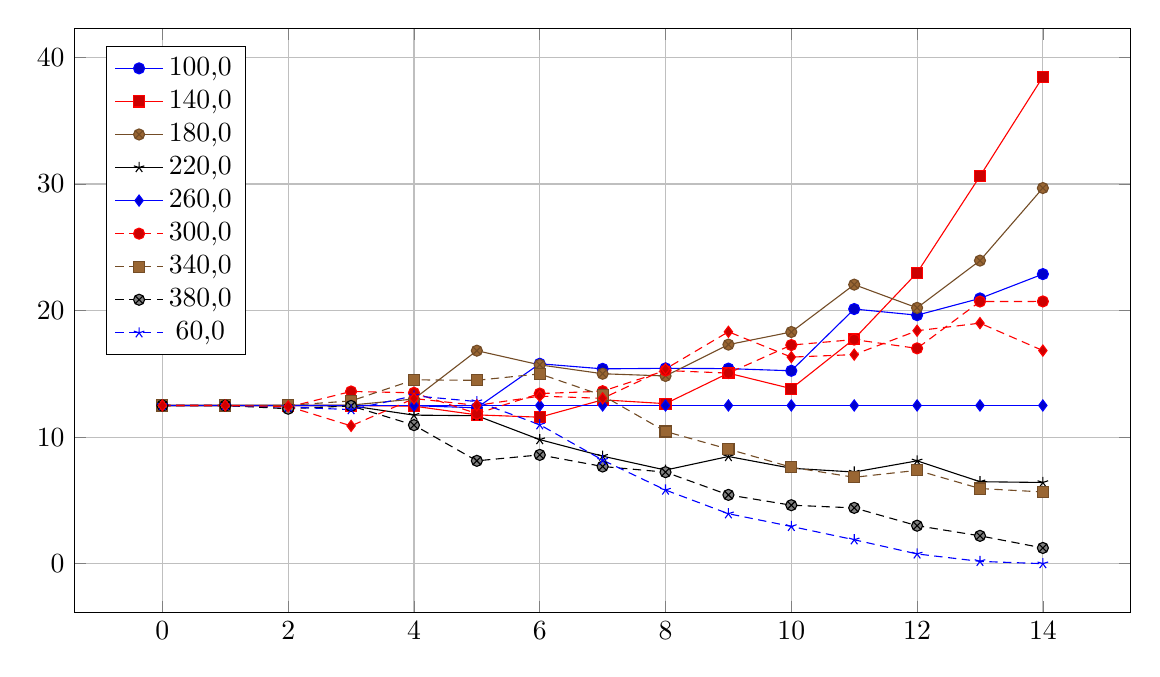
\begin{tikzpicture}
\begin{axis}[
height=9cm,
width=15cm,
grid=major,
legend style = { legend pos = north west }
]
\addplot coordinates {(0, 12.5 ) (1, 12.49999 ) (2, 12.499824 ) (3, 12.498202 ) (4, 12.481768 ) (5, 12.316477 ) (6, 15.795458 ) (7, 15.392218 ) (8, 15.434127 ) (9, 15.410436 ) (10, 15.239715 ) (11, 20.11805 ) (12, 19.633654 ) (13, 20.956968 ) (14, 22.878029 )};
\addlegendentry{100,0}
\addplot coordinates {(0, 12.5 ) (1, 12.499967 ) (2, 12.499719 ) (3, 12.496181 ) (4, 12.446304 ) (5, 11.755087 ) (6, 11.572497 ) (7, 12.945028 ) (8, 12.642736 ) (9, 15.052362 ) (10, 13.829583 ) (11, 17.761051 ) (12, 22.982285 ) (13, 30.615692 ) (14, 38.457775 )};
\addlegendentry{140,0}
\addplot coordinates {(0, 12.5 ) (1, 12.500086 ) (2, 12.501545 ) (3, 12.527953 ) (4, 13.00956 ) (5, 16.828875 ) (6, 15.706829 ) (7, 15.004946 ) (8, 14.830004 ) (9, 17.307192 ) (10, 18.304008 ) (11, 22.046404 ) (12, 20.210443 ) (13, 23.944548 ) (14, 29.67809 )};
\addlegendentry{180,0}
\addplot coordinates {(0, 12.5 ) (1, 12.499971 ) (2, 12.498856 ) (3, 12.470235 ) (4, 11.736132 ) (5, 11.689475 ) (6, 9.801909 ) (7, 8.49379 ) (8, 7.395703 ) (9, 8.466985 ) (10, 7.53862 ) (11, 7.24089 ) (12, 8.123841 ) (13, 6.475091 ) (14, 6.414579 )};
\addlegendentry{220,0}
\addplot coordinates {(0, 12.5 ) (1, 12.5 ) (2, 12.5 ) (3, 12.5 ) (4, 12.5 ) (5, 12.5 ) (6, 12.5 ) (7, 12.5 ) (8, 12.5 ) (9, 12.5 ) (10, 12.5 ) (11, 12.5 ) (12, 12.5 ) (13, 12.5 ) (14, 12.5 )};
\addlegendentry{260,0}
\addplot coordinates {(0, 12.499857 ) (1, 12.495675 ) (2, 12.370698 ) (3, 13.60359 ) (4, 13.500814 ) (5, 11.857204 ) (6, 13.439519 ) (7, 13.624933 ) (8, 15.260229 ) (9, 15.055403 ) (10, 17.272354 ) (11, 17.70488 ) (12, 17.010616 ) (13, 20.71158 ) (14, 20.718487 )};
\addlegendentry{300,0}
\addplot coordinates {(0, 12.5 ) (1, 12.500324 ) (2, 12.510459 ) (3, 12.8578205 ) (4, 14.523903 ) (5, 14.485657 ) (6, 14.996248 ) (7, 13.288555 ) (8, 10.443586 ) (9, 9.050881 ) (10, 7.6211677 ) (11, 6.8238263 ) (12, 7.3748183 ) (13, 5.9362407 ) (14, 5.6662164 )};
\addlegendentry{340,0}
\addplot coordinates {(0, 12.499819 ) (1, 12.493163 ) (2, 12.240214 ) (3, 12.464691 ) (4, 10.947274 ) (5, 8.125346 ) (6, 8.594709 ) (7, 7.6774254 ) (8, 7.2305574 ) (9, 5.434474 ) (10, 4.619633 ) (11, 4.406925 ) (12, 3.0008664 ) (13, 2.1981838 ) (14, 1.2431407 )};
\addlegendentry{380,0}
\addplot coordinates {(0, 12.499952 ) (1, 12.496996 ) (2, 12.374047 ) (3, 12.170701 ) (4, 13.262201 ) (5, 12.808096 ) (6, 10.978055 ) (7, 8.181279 ) (8, 5.8180957 ) (9, 3.9461956 ) (10, 2.943127 ) (11, 1.8900867 ) (12, 0.7694603 ) (13, 0.18109135 ) (14, 0.0 )};
\addlegendentry{60,0}
\addplot coordinates {(0, 12.499843 ) (1, 12.496562 ) (2, 12.424397 ) (3, 10.886884 ) (4, 13.046445 ) (5, 12.5084505 ) (6, 13.237075 ) (7, 13.062155 ) (8, 15.385118 ) (9, 18.319933 ) (10, 16.32064 ) (11, 16.517368 ) (12, 18.403559 ) (13, 19.003183 ) (14, 16.835337 )};
\end{axis}
\end{tikzpicture}


Z wyników można odczytać, że przy długości podkroku $ \frac{1}{260} $ sekundy
zasada zachowanaia energii zostaje spełniona. Okazuje się również, że wartość
tego parametru musi być odpowiednio dobrana(przy innych widoczne są
niedobory/nadmiary energii). Aby sprawdzić czy jest ona uniwersalna, kolejny
test zostanie przeprowadzony dla wartości prędkości 10$\frac{m}{s}$.

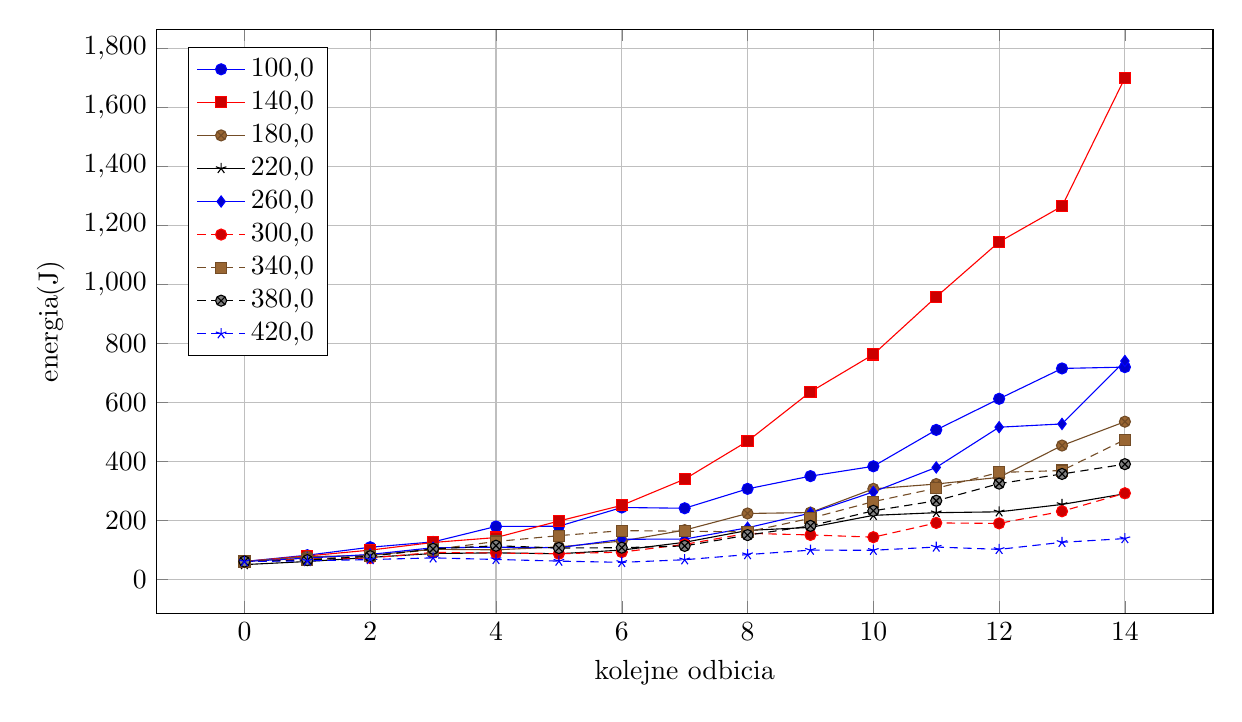
\begin{tikzpicture}
\begin{axis}[
height=9cm,
width=15cm,
grid=major,
xlabel=kolejne odbicia,
ylabel=energia(J),
legend style = { legend pos = north west }
]
\addplot coordinates {(0, 60.500023 ) (1, 81.92009 ) (2, 108.92922 ) (3, 126.9798 ) (4, 179.415 ) (5, 180.04378 ) (6, 243.66458 ) (7, 241.06052 ) (8, 306.84937 ) (9, 350.00568 ) (10, 383.3237 ) (11, 506.71848 ) (12, 612.16895 ) (13, 715.15283 ) (14, 719.6333 )};
\addlegendentry{100,0}
\addplot coordinates {(0, 60.5 ) (1, 79.38007 ) (2, 99.12363 ) (3, 125.07543 ) (4, 141.69774 ) (5, 197.75262 ) (6, 251.01779 ) (7, 339.7764 ) (8, 468.51224 ) (9, 635.6914 ) (10, 762.6489 ) (11, 957.757 ) (12, 1144.0896 ) (13, 1265.168 ) (14, 1700.5425 )};
\addlegendentry{140,0}
\addplot coordinates {(0, 60.50015 ) (1, 76.881676 ) (2, 81.42158 ) (3, 101.95011 ) (4, 100.09618 ) (5, 110.0021 ) (6, 129.7769 ) (7, 166.9779 ) (8, 223.40483 ) (9, 226.44267 ) (10, 306.8936 ) (11, 323.2172 ) (12, 345.97656 ) (13, 453.7002 ) (14, 534.60846 )};
\addlegendentry{180,0}
\addplot coordinates {(0, 50.0 ) (1, 60.499874 ) (2, 74.41864 ) (3, 87.634735 ) (4, 89.8731 ) (5, 86.80204 ) (6, 99.18527 ) (7, 125.629486 ) (8, 165.85115 ) (9, 176.15439 ) (10, 216.987 ) (11, 226.05557 ) (12, 228.96167 ) (13, 253.99066 ) (14, 290.1967 )};
\addlegendentry{220,0}
\addplot coordinates {(0, 60.500317 ) (1, 72.004326 ) (2, 84.55166 ) (3, 107.17797 ) (4, 109.10671 ) (5, 107.09075 ) (6, 135.90282 ) (7, 136.57355 ) (8, 174.91646 ) (9, 224.60782 ) (10, 296.45978 ) (11, 379.62122 ) (12, 515.9012 ) (13, 527.0016 ) (14, 740.21735 )};
\addlegendentry{260,0}
\addplot coordinates {(0, 60.500065 ) (1, 69.62055 ) (2, 72.48745 ) (3, 91.272835 ) (4, 89.28663 ) (5, 86.829384 ) (6, 92.37034 ) (7, 118.69746 ) (8, 156.08209 ) (9, 150.57904 ) (10, 143.00375 ) (11, 191.29128 ) (12, 189.68774 ) (13, 230.79619 ) (14, 292.0326 )};
\addlegendentry{300,0}
\addplot coordinates {(0, 60.500546 ) (1, 67.28903 ) (2, 80.538994 ) (3, 100.922035 ) (4, 128.30896 ) (5, 148.18803 ) (6, 165.16585 ) (7, 163.09677 ) (8, 161.04451 ) (9, 207.07037 ) (10, 263.59717 ) (11, 308.80777 ) (12, 362.447 ) (13, 368.95673 ) (14, 473.61365 )};
\addlegendentry{340,0}
\addplot coordinates {(0, 60.50036 ) (1, 64.98713 ) (2, 78.50689 ) (3, 103.256546 ) (4, 113.94582 ) (5, 106.305664 ) (6, 107.335 ) (7, 113.28537 ) (8, 150.0018 ) (9, 181.31984 ) (10, 232.42296 ) (11, 266.4738 ) (12, 324.6097 ) (13, 357.30115 ) (14, 390.61658 )};
\addlegendentry{380,0}
\addplot coordinates {(0, 60.50084 ) (1, 62.73556 ) (2, 67.12027 ) (3, 72.84919 ) (4, 67.44308 ) (5, 61.86573 ) (6, 57.622555 ) (7, 66.51577 ) (8, 83.97656 ) (9, 99.01908 ) (10, 98.68342 ) (11, 109.573204 ) (12, 101.67075 ) (13, 125.58686 ) (14, 138.26483 )};
\addlegendentry{420,0}
\end{axis}
\end{tikzpicture}


Jak widać odpowiednia wartość parametru \emph{fixedTimeStep} jest uzależniona od
wartości prędkości.

\subsubsection{Przypadek z wieloma ciałami}

TODO: dodać fragment o komentarzach w kodzie Bullet o wartościach friction i
restitution.

\subsection{Rzut ukośny}

\subsection{Równia pochyła}

\subsection{Zderzenie dwóch ciał}

\subsubsection{Zderzenie całkowicie sprężyste}

\subsubsection{Zderzenie całkowicie niesprężyste}

\subsection{Zderzenie trzech ciał}

\subsection{Odbicie podkręconej piłki}

\subsection{Kołyska Newtona}

\subsection{Ciało na sprężynie}

\subsection{Model ciała sprężystego}
